\subsection{Results}
\begin{frame}{}
	\LARGE VAE: \textbf{Results}
\end{frame}

\begin{frame}[allowframebreaks]{Results}
\begin{figure}
        \centering
        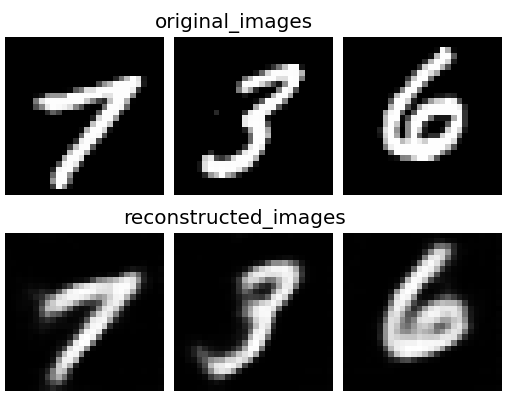
\includegraphics[height=0.8\textheight, width=\textwidth, keepaspectratio]{images/vae/result-mnist-1.png}
        \caption*{Image reconstruction with variational autoencoders on MNIST digits dataset}
\end{figure}

\framebreak
\begin{figure}
        \centering
        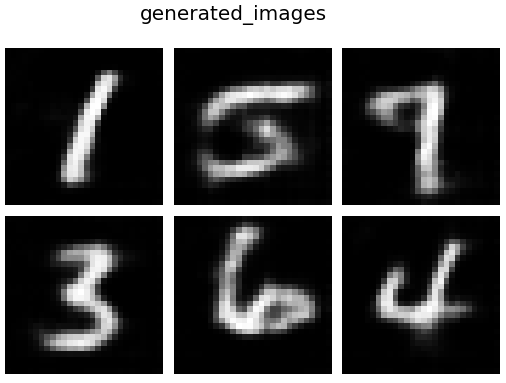
\includegraphics[height=0.8\textheight, width=\textwidth, keepaspectratio]{images/vae/result-mnist-2.png}
        \caption*{Image generation with variational autoencoders on MNIST digits dataset. Sample an encoding vector from $\mathcal{N}(0,1)$ and passed it through decoder}
\end{figure}

\framebreak

\begin{figure}
        \centering
        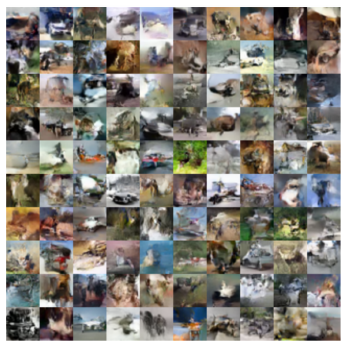
\includegraphics[height=0.8\textheight, width=\textwidth, keepaspectratio]{images/vae/result-cifar.png}
        \caption*{Image generation with variational autoencoders on CIFAR-10 32x32 dataset}
\end{figure}

\framebreak

\begin{figure}
        \centering
        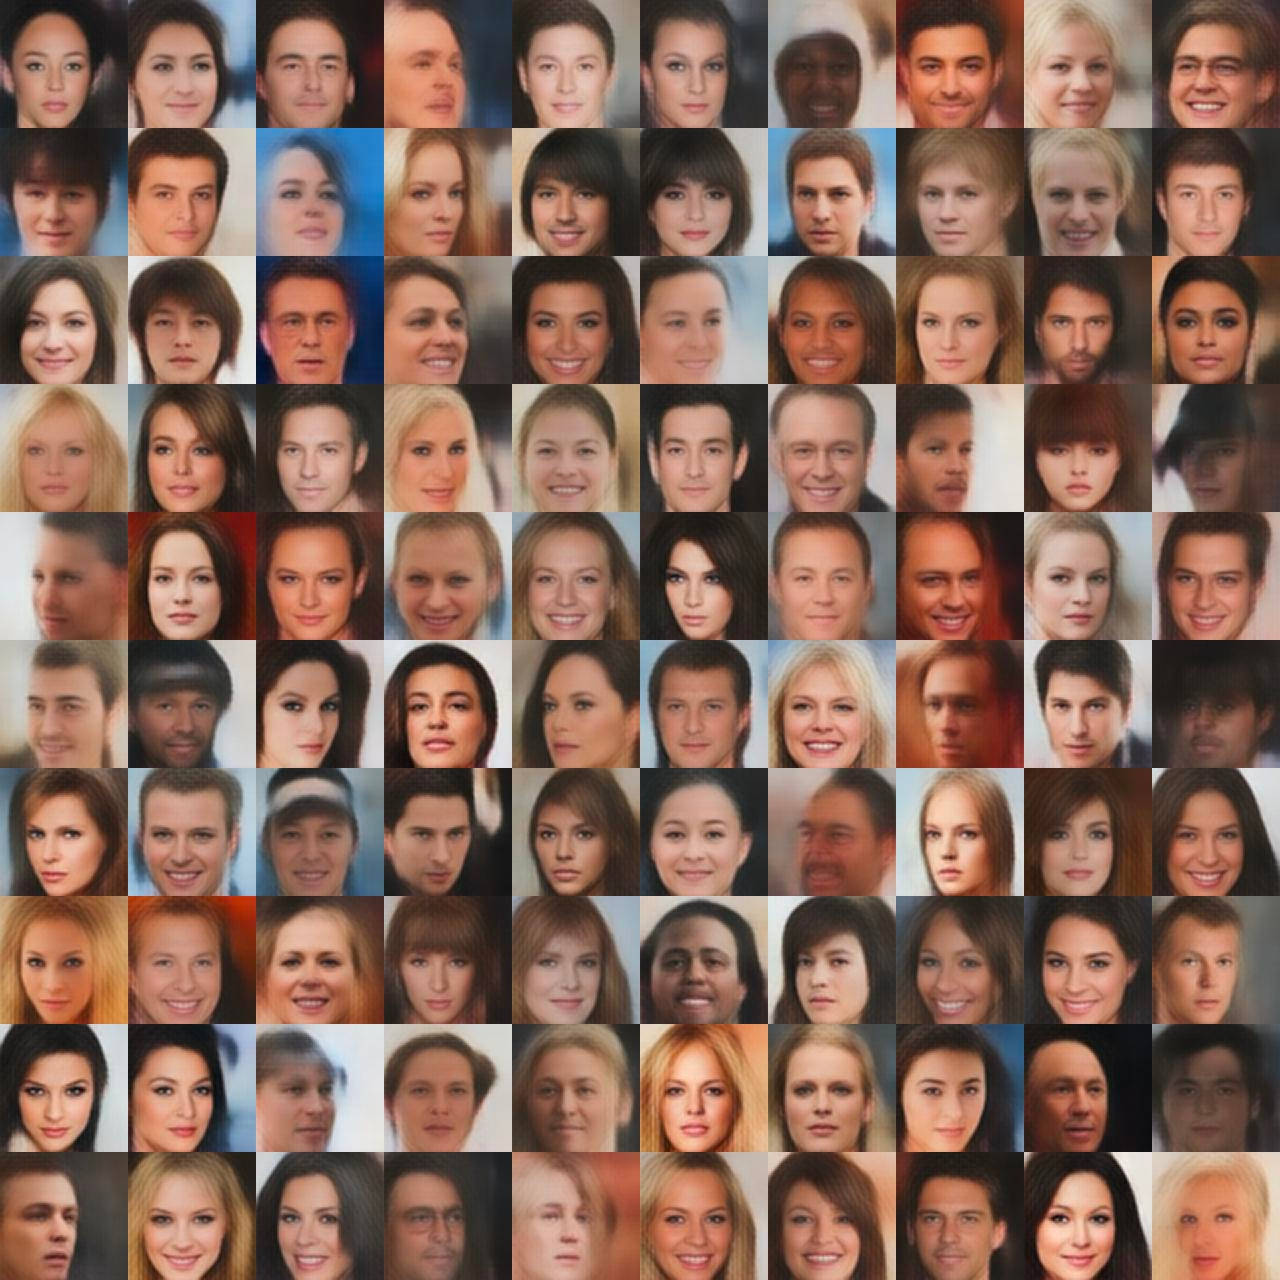
\includegraphics[height=0.8\textheight, width=\textwidth, keepaspectratio]{images/vae/result-face.png}
        \caption*{https://github.com/houxianxu/DFC-VAE}
\end{figure}
\end{frame}